\documentclass[11pt]{article}

\usepackage{url}
\usepackage{multicol}
\usepackage[english]{babel}
\usepackage[margin=1in]{geometry}
\usepackage{graphicx}
\usepackage{subcaption}
\usepackage{enumitem}
\usepackage{amsmath}
\usepackage{amssymb}
\usepackage{wasysym}
\usepackage{color}
\usepackage{float}
\usepackage{nomencl}
\usepackage[title]{appendix}
\makenomenclature
\usepackage{pdfpages}
\usepackage{algorithm}
\usepackage{algpseudocode}
\usepackage{hyperref}
\hypersetup{
    colorlinks=true,
    linkcolor=blue,
    filecolor=magenta,      
    urlcolor=cyan,
    pdftitle={Overleaf Example},
    pdfpagemode=FullScreen,
    }
\title{16-745 Optimal Control Lecture 19}
\author{Reid Graves} 

\begin{document}
\maketitle

\section*{Last Time}
\begin{itemize}
    \item Iterative Learning Control
\end{itemize}

\section*{Today}
\begin{itemize}
    \item Stochastic Optimal Control
\end{itemize}


\section*{Stochastic Control}
\begin{itemize}
    \item So far we have assumed we know the system's state perfectly
    \item What happens when all we have are noisy measurements of quantities related to the state?
    \begin{align*}
    \underbrace{y}_{\textcolor{cyan}{\text{measurements}}} &= \underbrace{g(x,v))}_{\textcolor{cyan}{\text{``measurement model"}}}
    \\
    &\text{where } v \text{ is noise}
    \end{align*}
    \begin{align*}
        & \underline{\text{Deterministic}} & &\underline{\text{Stochastic}}
        \\
        & \hspace{10mm} x  \hspace{15mm}\rightarrow &&\hspace{5mm}  p(x|y)\textcolor{cyan}{\leftarrow\text{ PDF if the state conditioned on measurements}}
    \end{align*}
\end{itemize}


\subsection*{Stochastic Optimal control problem}
\begin{align*}
    \min_u \quad E[J(x,u)]
\end{align*}
\begin{itemize}
    \item In principle, can solve with DP
    \item Very hard in general
\end{itemize}

\subsection*{Linear Quadratic Gaussian (LQG)}
\begin{itemize}
    \item Special case we can solve in closed form:
    \begin{align*}
        &\underline{\text{L}}\text{inear Dynamics}
        \\
        &\underline{\text{Q}}\text{uadratic Cost} 
        \\
        &\underline{\text{G}}\text{aussian Noise}
    \end{align*}
    \item Dynamics
    \begin{align*}
        x_{k+1} &= Ax_k + Bu_k + w_k\textcolor{cyan}{\leftarrow\text{``process noise"}} \\
        y_k &= Cx_k + v_k\textcolor{cyan}{\leftarrow\text{``Measurement noise"}}
    \end{align*}
    \begin{align*}
        w_k &\sim N(0,W) & v_k&\sim N(0,V)
    \end{align*}
    where $\sim$ is ``drawn from", $N$ is Normal Gaussian distribution, 0 is mean, and $W,V$
 is covariance
 \end{itemize}

 \subsection*{Multivariate Gaussian}
 \begin{align*}
     p(x) &= \frac{1}{\sqrt{(2\pi)^k det(S)}}exp(-\frac{1}{2}(x-\mu)^TS^{-1}(x-\mu))
     \\
     \text{mean: } \mu &= \hat{x} = E[x] \in \mathbb{R}^n  
     \\
     \text{covariance: } S &= E[(x-\mu)(x-\mu)^T] \in S_{tt}^n
     \\
     E[f(x)] &= \int_\text{(all space)}f(x) p(x) dx
     \\
     \text{``Uncorrelated"} &\Rightarrow E[(x-\hat{x})(y-\hat{y})^T] = 0
 \end{align*}
 Where $S$ is the covariance matrix, 

 \begin{itemize}
     \item Cost function
     \begin{align*}
         J &= E\left[\frac{1}{2}x_N^TQx_N + \frac{1}{2}\sum_{k=1}^{N-1} (x_k^TQx_k + u_k^TRu_k)\right]
     \end{align*}
     \item D.P. Recursion
     \begin{align*}
         V_N(x) &= \frac{1}{2}E[x_N^TQx_N] = \frac{1}{2}E[x_N^TP_Nx_N]
         \\
         V_{N-1}(x) &= \min_u E\Big[\frac{1}{2}x_{N-1}^TQx_{N-1} + \frac{1}{2}u_{N-1}^TRu_{N-1} + \frac{1}{2}(Ax_{N-1} + Bu_{N-1} \\ & + w_{N-1})^TP_N(Ax_{N-1} + Bu_{N-1} + w_{N-1})\Big] 
         \\
         &= \min_u \underbrace{E\left[\frac{1}{2}x_{N-1}^TQx_{N-1} + \frac{1}{2} u_{N-1}^TRu_{N-1} + (Ax_{N-1} + Bu_{n-1})^TP_N(Ax_{N-1} + Bu_{N-1})\right]}_{\textcolor{cyan}{\text{Standard LQR}}} 
         \\
         & + \underbrace{E\left[ \underbrace{(Ax_{N-1} + Bu_{N-1})^T}_{\textcolor{red}{0}}w_{N-1}+ w_{N-1}^TP_N\underbrace{(Ax_{N-1} + Bu_{N-1})}_{\textcolor{red}{0}} +\underbrace{w_{N-1}P_Nw_{N-1}}_{\textcolor{green}{Constant!}} \right]}_{\textcolor{cyan}{\text{Noise Terms}}}
     \end{align*}
     \textcolor{red}{Noise sample drawn at time K has nothing to do with state (or control) at time k. $x_k$ depends on $w_{k-1}$ (and all past w) but not on $w_k$ or future $w$}
     \begin{align*}
         &\textcolor{red}{\Rightarrow \text{ Uncorrelated } \Rightarrow \text{cross-correlation is zero}}
         \\
        & \Rightarrow \text{Noise terms have no impact on the controller design! (you just get a higher cost)}
     \end{align*}
 \end{itemize}

 \subsection*{``Certainty-Equivalence Principle"}
 \begin{itemize}
     \item The optimal LQG controller is just LQR with x replaced by E[x]
 \end{itemize}

 \subsection*{``Separation Principle"} 
 \begin{itemize}
     \item For LQG we can design an optimal feedback controller and an optimal estimator separately and then hook them together. The resulting feedback policy is optimal.
 \end{itemize}

 \subsection*{Neither of these holds in general but are still frequently used in practice to design sub-optimal policies}

 \subsection*{Optimal state Estimation:}

 \begin{itemize}
     \item What should I try to optimize?
     \begin{figure}[H]
         \centering
         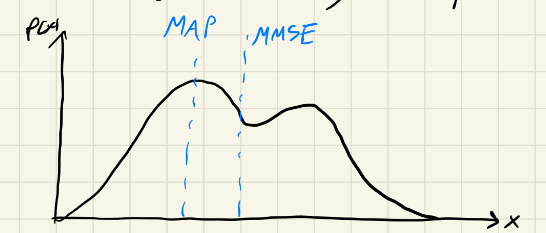
\includegraphics[width=0.5\linewidth]{lecture_19_1.png}
     \end{figure}
     \item Maximum a-posterior: (MAP):
     \begin{align*}
         argmax\quad p(x|y)
     \end{align*}
     \item Minimum mean-squared error(MMSE):
     \begin{align*}
         argmin\quad E[{(x-\hat{x})^T(x-\hat{x})}]
     \end{align*}
     \item These are the same for a Gaussian!
 \end{itemize}



\end{document}
